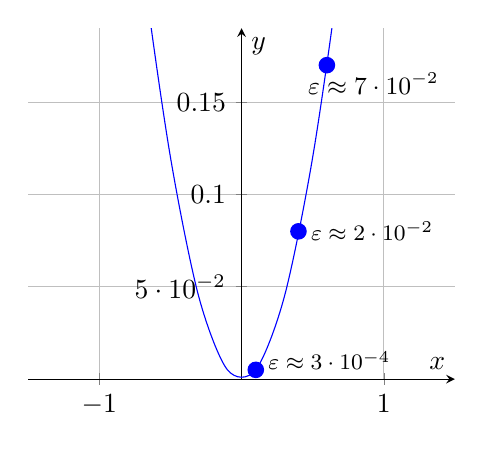
\begin{tikzpicture}
\begin{axis}[
    width=7cm,
    xlabel={$x$},
    ylabel={$y$},
    xmin=-1.5, xmax=1.5,
    ymin=0, ymax=0.19, % Adjust y-axis limits
    axis lines=center,
    grid=both,
    domain=-10:10,
    samples=100,
    % restrict y to domain=-2.5:2.5 % Restrict y-axis domain
]

\addplot[blue, smooth] {ln(cosh(x))};

\coordinate (A1) at (axis cs:0.6,0.17);
\coordinate (B1) at (axis cs:0.4,0.16);

\fill[blue, thick] (A1) circle (3pt);
\node[right] at (B1) {\small $\bm{\varepsilon \approx 7 \cdot 10^{-2}}$};

%\draw[dashed] (A1) -- (B1);
 %----------------------------------------%
\coordinate (A2) at (axis cs:0.4,0.08);
\coordinate (B2) at (axis cs:0.42,0.08);

\fill[blue, thick] (A2) circle (3pt);
\node[right] at (B2) {\footnotesize $\bm{\varepsilon \approx 2 \cdot 10^{-2}}$};

%\draw[dashed] (A2) -- (B2);
 %----------------------------------------%
% \coordinate (A3) at (axis cs:0.2,0.02);
% \coordinate (B3) at (axis cs:0.35,0.03);

% \fill[blue, thick] (A3) circle (3pt);
% \node[right] at (B3) {\footnotesize $\bm{\varepsilon \approx 2 \cdot 10^{-3}}$};

% \draw[dashed] (A3) -- (B3);
%----------------------------------------%
\coordinate (A4) at (axis cs:0.1,0.005);
\coordinate (B4) at (axis cs:0.12,0.01);

\fill[blue, thick] (A4) circle (3pt);
\node[right] at (B4) {\footnotesize $\bm{\varepsilon \approx 3 \cdot 10^{-4}}$};

%\draw[dashed] (A4) -- (B4);

\end{axis}
\end{tikzpicture}